\documentclass[mathserif,handout]{beamer}
\definecolor{red}{rgb}{1,0,0}
\definecolor{bulletcolor}{rgb}{0,0,1}
\usetheme{Madrid}
\usepackage{amssymb}
\usepackage[utf8x]{inputenc}     % Mapea Caracteres Latinos.
\usepackage[spanish]{babel}       % Hyphenation patterns as the base language is switched.
\usepackage{pdfpages}
\usepackage{pgfplots}
\usepackage{tikz}
\usetikzlibrary{shapes}
\usetikzlibrary{positioning}
\usetikzlibrary{intersections}

\spanishdecimal{.}

\makeatletter
\setbeamertemplate{footline}
{
  \leavevmode%
  \hbox{%
  \begin{beamercolorbox}[wd=.333333\paperwidth,ht=2.25ex,dp=1ex,center]{author in
  head/foot}%
    \usebeamerfont{author in head/foot}\insertshortauthor%~~\beamer@ifempty{\insertshortinstitute}{}{(\insertshortinstitute)}
  \end{beamercolorbox}%
  \begin{beamercolorbox}[wd=.333333\paperwidth,ht=2.25ex,dp=1ex,center]{title in
  head/foot}%
    \usebeamerfont{title in head/foot}\insertshorttitle
  \end{beamercolorbox}%
\begin{beamercolorbox}[wd=.333333\paperwidth,ht=2.25ex,dp=1ex,center]{date in
   head/foot}%
    \usebeamerfont{subtitle in head/foot}\insertsubtitle{}
  \end{beamercolorbox}
  }%
  \vskip0pt%
}
\makeatother

\setbeamertemplate{navigation symbols}{}%remove navigation symbols
\newcommand{\tab}[1]{\hspace{.2\textwidth}\rlap{#1}}

\newcommand{\sectionstart}[2]{
\section{#1}
\label{sec:#2}

\begin{frame}{}
  \begin{center}
    \begin{LARGE}
      \textbf{\ref{sec:#2}. #1}
    \end{LARGE}
  \end{center}
\end{frame}
}

\newcommand{\N}{\mathbb{N}}
\newcommand{\Exp}[1]{\mathcal{E}_{#1}}
\newcommand{\EN}{\Exp{\N}}
\newcommand{\lb}{\\~\\}

\begin{document}
\title{Taller de Programación Avanzada}
\subtitle{Introducción}
\author[Gabriel Diéguez Franzani]
{%
\centering
Gabriel Diéguez Franzani\\
\href{mailto:gsdieguez@ing.puc.cl}{gsdieguez@ing.puc.cl}
  }

\date{\lb 17 de marzo de 2017}

\institute{\lb Departamento de Ciencia de la Computación\\ Escuela de
Ingeniería\\
Pontificia Universidad Católica de Chile}

%Sacar footline a páginas iniciales
{
	\setbeamertemplate{footline}{}
	\frame{\titlepage}
}

\section{Información general}

\begin{frame}{Información General}
\begin{center}
    \begin{tabular}{r  l}
		\multicolumn{2}{c}{} \\
		\textbf{Sigla:} & IIC2252 \\
		\textbf{Nombre:} & Taller de Programación Avanzada \\\pause
		\textbf{Profesor:} & Gabriel Diéguez Franzani (gsdieguez@ing.puc.cl)\\\pause
		\textbf{Ayudante:} & Pablo Messina (pamessina@uc.cl)\\\pause
		\textbf{Horario:} & V:4-6, Sala Javier Pinto\\\pause
		\textbf{Sitio Web:} & Siding y Github del curso
    \end{tabular}
    \end{center}
\end{frame}

\begin{frame}{Introducción}
  \begin{center}
    \huge Programación Competitiva
  \end{center}
\end{frame}

\begin{frame}{Introducción}

\begin{center}

\includegraphics[width=10cm]{acm_icpc}
\end{center}
\end{frame}

\begin{frame}{Introducción}

\begin{center}
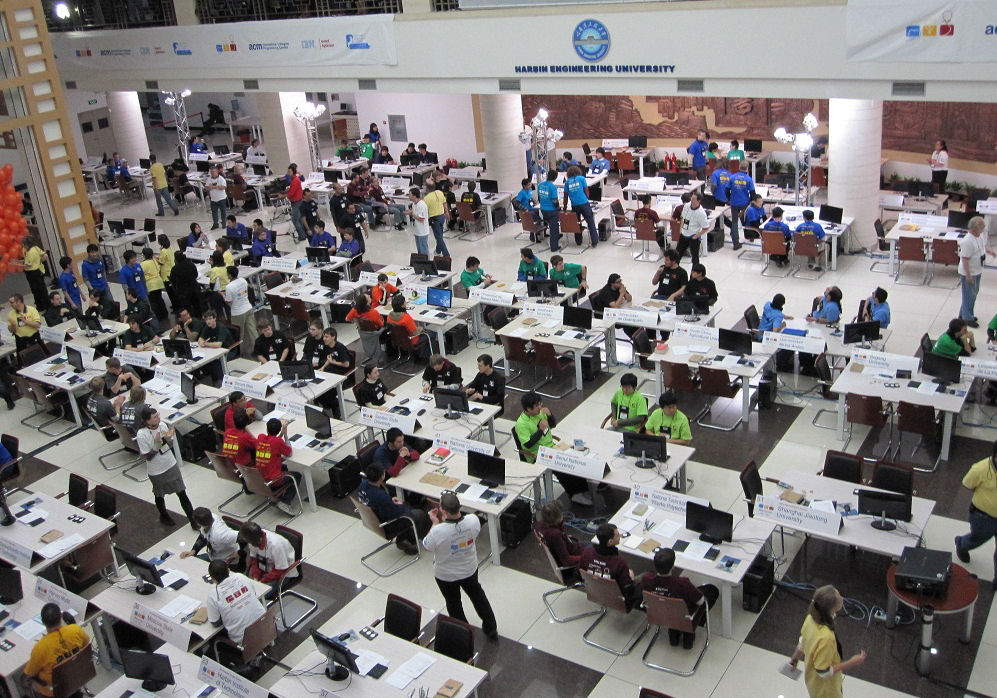
\includegraphics[width=10cm]{icpc-contest}
\end{center}
\end{frame}

\begin{frame}{Introducción}

\begin{center}
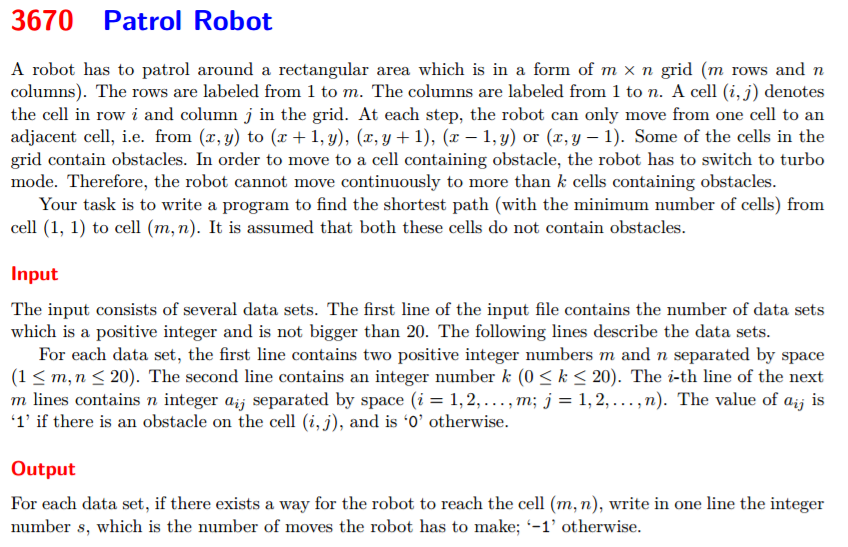
\includegraphics[width=10cm]{problema}
\end{center}
\end{frame}

\begin{frame}{Introducción}
  \begin{itemize}
      \item Estructuras de datos\pause
      \item Búsqueda\pause
      \item Grafos\pause
      \item Programación dinámica\pause
      \item Strings\pause
      \item Geometría
\end{itemize}
\end{frame}

\begin{frame}{Metodología}
  \begin{itemize}
    \item Dos tipos de clases:\pause
    \begin{enumerate}
      \item Teórico-prácticas: habrá una pequeña clase sobre algún tópico, y luego un set de problemas temático.\pause
      \item 100\% prácticas: habrá un set de problemas (temático o no) a resolver.\pause
    \end{enumerate}

      \item Los problemas son evaluados por jueces automáticos.\pause
      \item Pueden desarrollar los sets en grupos (no más de 3 personas), pero cada uno debe enviar sus respuestas.\pause
      \item Lenguajes permitidos: C++, Java, Python.
\end{itemize}
\end{frame}

\begin{frame}{Evaluación}
  \begin{itemize}
      \item Todos parten con un 7 :D\pause
      \item Para mantenerlo, deben tener un 100\% de asistencia :(\pause
      \item Se considerará presente a quien:\pause
      \begin{enumerate}
        \item Resuelva al menos un problema durante las clases teórico-prácticas, o\pause
        \item Resuelva al menos dos problemas durante las clases 100\% prácticas, o\pause
        \item Resuelva al menos tres problemas de manera remota (los contests estarán disponibles durante toda la semana).
      \end{enumerate}
\end{itemize}
\end{frame}

\begin{frame}
  \frametitle{}
  \begin{center}
    \huge ¿Preguntas?
  \end{center}
\end{frame}

{
	\setbeamertemplate{footline}{}
	\frame{\titlepage}
}

\end{document}
